\documentclass[a4paper, 12pt]{article}

\usepackage{cmap}
\usepackage[T2A]{fontenc}
\usepackage[english, russian]{babel}
\usepackage[utf8]{inputenc}
\usepackage[left=2cm,right=1.5cm,top=2cm,bottom=2cm]{geometry}
\usepackage{amsmath}
\usepackage{amssymb}
\usepackage{etoolbox}
\usepackage{amsthm}
\usepackage{booktabs}
\usepackage{graphicx}
\usepackage{tikz}
\usetikzlibrary{arrows}

\newcommand{\Z}{\mathbb{Z}}
\newcommand{\N}{\mathbb{N}}
\newcommand{\R}{\mathbb{R}}
\newcommand{\Q}{\mathbb{Q}}
\renewcommand{\phi}{\varphi}
\renewcommand{\epsilon}{\varepsilon}
\newcommand{\lra}{\Leftrightarrow}
\renewcommand{\emptyset}{\varnothing}
\newcommand\tab[1][.5cm]{\hspace*{#1}}
\newcommand{\hsp}{\hspace{5pt}}
\newcommand{\om}{\bar{\bar{o}}}

\theoremstyle{definition}
\newtheorem*{definition}{Определение}
\newtheorem*{theorem}{Теорема}
\newtheorem*{consequense}{Следствие}
\newtheorem*{lemma}{Лемма}
\newtheorem*{comm}{Замечание}
\newtheorem*{statement}{Утверждение}
\newtheorem*{example}{Пример}
\newtheorem*{examples}{Примеры}
\newtheorem*{axiom}{Аксиома}

\usepackage{titlesec}
\titleformat{\section}{\LARGE \bfseries}{\thesection}{1em}{}
\titleformat{\subsection}{\Large\bfseries}{\thesubsection}{1em}{}
\titleformat{\subsubsection}{\large\bfseries}{\thesubsubsection}{1em}{}

\usepackage{hyperref}
\usepackage{xcolor}
\definecolor{linkcolor}{HTML}{225ae2}
\definecolor{urlcolor}{HTML}{225ae2}
\hypersetup{
    pdfstartview=FitH, 
    linkcolor=linkcolor,
    urlcolor=urlcolor,
    colorlinks=true
}

\title{\textbf{Математический анализ-1}}
\author{Лектор: Подольский Владимир Евгеньевич}

\begin{document}
    \fontsize{14pt}{20pt}\selectfont
    \maketitle
    \vspace{0.3cm}
    \begin{center}
        
\includegraphics[width=0.8\linewidth]{mehmat.png}
    \end{center}
    \vspace{1.5cm}
    \begin{center}
        Конспект: Кирилл Яковлев, 108 группа \tab[5.5cm] tg: @fourkenz
    \end{center}
    \newpage
    \tableofcontents
    \fontsize{14pt}{20pt}\selectfont
    \newpage

    \section{Элементы теории множеств}
    \subsection{Условности и обозначения}
        \begin{definition}
            Кванторами будем назать символы, заменяющие слова в выражениях.
        \end{definition}
        \begin{comm}
            Пока что кванторы не подразумевают логические операции, мы будем использовать их только для более удобной и формальной записи.
        \end{comm}
        \begin{itemize}
            \item $\forall$ - квантор всеобщности
            \item $\exists$ - квантор существования
            \item $!$ - квантор единственности
            \item Запись $A \Rightarrow B$ обозначает, что из высказывания $A$, следует высказывание $B$. 
            \item Запись $A \lra B$ обозначает, что высказывание $A$ равносильно высказыванию $B$.
            \item Запись $a \in A$ означает, что $a$ является элементом множества $A$, отрицанием такой записи будет $a \notin A$
            \item Если $x$ - объект, а $P$ - свойство, то запись $\{x : P(x)\}$ означает класс всех объектов обладающих свойством $P$.
        \end{itemize}
        \begin{definition}
            Множество не содержащее ни одного элемента называется пустым и обозначается $\emptyset$.
        \end{definition}
        \begin{definition}
            Множество $A^{\prime}$ является подмножеством множества $A$, \\ если $\forall a: a\in A^{\prime}\Rightarrow a\in A$. Запись $A^{\prime} \subset A$ обозначает, что $A^{\prime}$ является подмножеством $A$.
        \end{definition}        
        \begin{definition}
            Для любого множества $A$ выполнено:
            \begin{enumerate}
                \item $\emptyset \subset A$.
                \item $A \subset A$.
            \end{enumerate}
        \end{definition}
        \begin{definition}
            Если $A\subset B$ и $A\ne B$, то $A$ называется собственным подмножеством множества $B$.
        \end{definition}
    \subsection{Операции над множествами}
        \begin{definition}
            Множество $C=A\cup B$ называется объединением множеств $A$ и $B$, если $\forall a: (a\in A \Rightarrow a\in C)$ и $\forall b: (b\in B\Rightarrow b\in C)$, а также $\forall c: c\in C \Rightarrow (c\in A$ или $c\in B)$.        \end{definition}
        \begin{definition}
            Множество $C=A\cap B$ называется пересечением множеств $A$ и $B$, если $\forall c: c\in C \Rightarrow (c\in A$ и $c\in B)$, а также $\forall c: (c\in A$ и $c\in B) \Rightarrow c\in C$.        \end{definition}
        \begin{definition}
            Множество $C=A\setminus B$ называется разностью множеств $A$ и $B$, если $\forall c: (c\in A$ и $c\not\in B) \Rightarrow c\in C$, а также $\forall c: c\in C \Rightarrow (c\in A$ и $c\not\in B)$
        \end{definition}
        \begin{statement}
            $A\cup(B\cap C)=(A\cup B)\cap(A\cup C)$.
        \end{statement}
        \begin{proof} 
            $a\in (A\cup(B\cap C)) \lra a\in A$ или $a\in (B\cap C) \lra a\in A$ или $(a\in B$ и $a\in C) \lra (a\in A$ или $a\in B)$ и $(a\in A$ или $a\in C)$.
        \end{proof}
        \begin{statement}
            $A\cap(B\cup C)=(A\cap B)\cup(A\cap C)$.
        \end{statement}
        \begin{proof}
            $a\in (A\cap(B\cup C)) \lra a\in A$ и $a\in (B\cap C)\lra a\in A$ и \\ $(a\in B$ или $a\in C)\lra (a\in A$ и $a\in B)$ или $(a\in A$ и $a\in C)$.
        \end{proof}
    \subsection{Декартово произведение множеств}
        \begin{definition}
            Множество $A$ называется одноэлементным, если $\exists a\in A$ такое, что $A\setminus\{a\} = \emptyset$.
        \end{definition}
        \begin{definition}
            Множество $A$ называется двуэлементным, если $\exists a\in A$ такое, что $A\setminus\{a\}$ - одноэлементное.
        \end{definition}
        \begin{definition}
            Пусть $x\in X, y\in Y$. Упорядоченной парой называется двуэлементное множество $\{x,\{x,y\}\}$, упорядоченную пару обозначают $(x,y)$.
        \end{definition}
        \begin{definition}
            Множество всех упорядоченных пар $(x,y)$ называется декартовым произведением множеств $X$ и $Y$, где $x\in X, y\in Y$. Декартово произведение обозначают $X\times Y$.
        \end{definition}
    \subsection{Отображения}
        \begin{definition}
            Пусть $X, Y$ - множества. Подмножество $f\subset X\times Y$ такое, что $\forall\ (x_1,y_1),\ (x_2, y_2)\in f: y_1\ne y_2 \Rightarrow x_1\ne x_2$ называется отображением из $X$ в $Y$, и обозначается $f: X\to Y$.
        \end{definition}
        \begin{comm}
            Запись $(x,y)\in f$ часто заменяют на $y=f(x)$.
            \end{comm}
        \begin{definition}
            Пусть $f:X\to Y$. Множество $\{x: \exists\ (x,y) \in f\} = D_f$ называется областью определения функции $f$.
        \end{definition}
        \begin{definition}
            Пусть $f:X\to Y$. Множество $\{y: \exists\ (x,y) \in f\} = R_f$ называется областью значений функции $f$.
        \end{definition}
        \begin{definition}
            Пусть $f:X\to Y$. $f$ - инъекция $\lra \forall\ (x_1,y_1),\ (x_2,y_2)\in f: \\ x_1\ne x_2 \Rightarrow y_1\ne y_2$.
        \end{definition}
        \begin{definition}
            Пусть $f:X\to Y$. $f$ - сюръекция $\lra Y=R_f$
        \end{definition}
        \begin{comm}
        Обычно используют определение $f$ - сюръекция $\lra \forall y\in Y \\ \exists\ x\in X: y=f(x)$.
        \end{comm}
        \begin{definition}
            $f$ - биекция $\lra f$ - инъекция и $f$ - сюръекция.
        \end{definition}
        \begin{definition}
            Пусть $f:X\to Y,\ X_1\subset X$. Множество $\{(x,y)\in f: x\in X_1\}=f|\begin{matrix}
                \null \\ X_1
            \end{matrix}$ называется ограничением $f$ на $X_1$.
        \end{definition}
        \begin{definition}
            Пусть $f:X\to Y,\ X_1\subset X$. Множество $f(X_1)=\\ \{y\in Y: \exists\ x\in X_1 : (x,y)\in f\}$ называют образом множества $X_1$.
        \end{definition}
        \begin{definition}
            Пусть $f:X\to Y,\ Y_1\subset Y$. Множество $f^{-1}(Y_1)=\\ \{x\in X: \exists\ y\in Y_1 : (x,y)\in f\}$ называют полным прообразом множества $Y_1$.
        \end{definition}
        \begin{definition}
            Пусть $f:X\to Y$. Если $\forall y\in R_f: f^{-1}(y)$ - одноэлементное множество, то подмножество $f^{-1}\subset Y\times X=\{(y,x)\}$ является отображением и называется обратным отображением к $f$. Если у отображения $f$ существует обратное отображение $f^{-1}$, то оно называется обратимым.
        \end{definition}
        \begin{statement}
            $f$ - обратимое $\lra f$ - биекция.
        \end{statement}
        \begin{comm}
        Иногда $f: X\to Y$ записывают в виде $y_x$ и называют индексацией $y$ элементами $x$.
        \end{comm}
    \subsection{Операции над множествами (продолжение)}
        \begin{statement}
            $\bigcup\limits_{\alpha}(A\setminus A_{\alpha}) = A\setminus (\bigcap\limits_{\alpha}A_{\alpha})$.
        \end{statement}
        \begin{proof}
            $a\in \bigcup\limits_{\alpha}(A\setminus A_{\alpha})\lra (a\in A$ и $a\notin A_{\alpha_1})$ или $\dots$ или $(a\in A$ и $a\notin A_{\alpha_n})\lra a\in A$ и $(a\notin A_{\alpha_1}$ и $\dots$ и $a\notin A_{\alpha_n})\lra a\in A\setminus (\bigcap\limits_{\alpha}A_{\alpha})$.
        \end{proof}
        \begin{statement}
            $\bigcap\limits_{\alpha}(A\setminus A_{\alpha}) = A\setminus (\bigcup\limits_{\alpha}A_{\alpha})$.
        \end{statement}
        \begin{proof}
            $a\in \bigcap\limits_{\alpha}(A\setminus A_{\alpha})\lra (a\in A$ и $a\notin A_{\alpha_1})$ и $\dots$ и $(a\in A$ и $a\notin A_{\alpha_n})\lra a\in A$ и $(a\notin A_{\alpha_1}$ или $\dots$ или $a\notin A_{\alpha_n})\lra a\in A\setminus (\bigcup\limits_{\alpha}A_{\alpha})$.
        \end{proof}
    \section{Действительные числа}
    \subsection{Натуральные числа. Аксиоматика Пеано}
        \begin{definition} (Аксиоматика Пеано)
            \begin{enumerate}
                \item В множестве $\N$ $\forall n\in \N, \exists !$ элемент называемый следующим и обозначающийся как $S(n)$.
                \item $\forall n\in \N$ $\exists$ не более одного элемента $\N$, для которого $n$ - следующий.
                \item $\exists !$ элемент $\N$ не являющийся следующим ни для какого элемента. Этот элемент обозначается $1$ и называется единицей.
                \item (Аксиома индукции) Пусть $M\subset \N$, такое, что $1\in M$ и $\forall m\in M:\\ S(m)\in M$. Тогда $M=\N$.
            \end{enumerate}
        Множество удовлетворяющее этим аксиомам называется множеством натуральных чисел и обозначается $\N$.
        \end{definition}
        \begin{definition}
            Рассмотрим  множество $X$. Если для некоторого $n\in \N$ $\exists$ биекция $\phi: X\to \{1, \dots n\}$, то $X$ называется $n$-элементным, или говорят, что количество элементов в $X$ равно $n$. Тот факт что множество $X$ - $n$-элементное обозначается как $|X|=n$ или $cardX=n$.
        \end{definition} 
        \begin{comm}
            По определению считаем, что $card(\emptyset) =0$.
        \end{comm}
        \begin{definition}
            Все множества, количество элементов которых равно какому-то натуральному числу или нулю, называются конечными. Все остальные множетсва называются бесконечными.
        \end{definition}
    \subsection{Отношение порядка и принцип наименьшего элемента}
        \begin{definition}
            $R\subset X\times Y$ называется отношением между элементами\\ $X$ и $Y$. Обозначают $xRy$, если $(x,y)\in R$.
        \end{definition}
        \begin{definition}
            Отношение $R$ называется отношением порядка, если выполнено:
            \begin{enumerate}
                \item $\forall x,y: xRy$ или $yRx$. 
                \item Если верно $xRy$ и $yRx$, то $x=y$. 
                \item Если $xRy$ и $yRz$, то $xRz$.
            \end{enumerate}
            Такое отношение обозначают $\leq$.
        \end{definition}
        \begin{theorem}
            $\exists !$ отношение порядка на $\N$, такое, что $\forall n\in \N: n\leq S(n)$. (Можно использовать на экзамене без доказательства)
        \end{theorem}
        \begin{theorem} (Принцип наименьшего элемента)\\
            $M\subset \N, M\ne \emptyset$ имеет наименьшей элемент, т.е. $\exists n_{min}\in M, \forall n\in M: n_{min}\leq n$.
        \end{theorem} 
        \begin{proof}
            База: Если $1\in M$, то $n_{min}=1$. Пусть $1\notin M$, тогда $1\in \N\setminus M$.\\
            Шаг: Пусть $\{1,2,\dots, n\}\subset \N\setminus M$. Тогда $S(n)\in \N\setminus M\Rightarrow$ по аксиоме индукции $\N\setminus M=\N\Rightarrow M = \emptyset$ - противоречие.
        \end{proof}
    \subsection{Арифметические операции}
        \begin{definition}
            Рассмотрим $A,B, card(A)=n, card(B)=k, n,k\in \N$. Пусть $A\cap B=\emptyset$. Тогда число $card(A\cup B)$ называется суммой $n$ и $k$ и обозначается $card(A\cup B)=n+k$.
        \end{definition}
        \begin{comm}
            Естественно выполняется $n+k=k+n$ (коммутативность) и\\ $(n+k)+m=n+(k+m)$ (ассоциативность).
        \end{comm}
        \begin{comm}
            $n+0=0+n=n$, т.к. $cardA=card(A\cup \emptyset)$.
        \end{comm}
        \begin{comm}
            $A \leftrightarrow \{1,\dots, n\}, B\leftrightarrow \{1,\dots, k\}$. Возьмем\\ $card(A\cup B)=\{1,\dots, n\}\cup \{\underbrace{S(n), S(S(n)), \dots, S(S(\dots (S(n))\dots)}_k\}$,\\ (где $\{1,\dots, k\} \leftrightarrow \{\underbrace{S(n), S(S(n)), \dots, S(S(\dots (S(n))\dots)}_k\}) \Rightarrow S(n)=n+1$.
        \end{comm} 
        \begin{definition}
            $n,k\in \N$. Тогда $\sum\limits_{i=1}^kn=nk$ называется произведением $n$ на $k$.
        \end{definition}
        \begin{comm}
            $nk=\underbrace{(n+n+\dots +n)}_k$. 
        \end{comm}
        \begin{comm} Выполнены:
            \begin{itemize}
                \item $nk=kn$ (коммутативность)
                \item $n(km)=(nk)m$ (ассоциативность)
                \item $k(n+m)=kn+km$ (дистрибутивность)
                \item Если $k\leq n$, то $k+m\leq n+m$ и если $k\leq m$, то $kn\leq mn$
            \end{itemize}
        \end{comm}
        \begin{definition}
            Если $n+k=m$, то $n=m-k$ называется разностью\\ $m$ и $k,\ k=m-n$ называется разностью $m$ и $n$.
        \end{definition}
        \begin{comm}
            $m-0=m$, $m+0=m$, $m-m=0$.
        \end{comm}
        \begin{definition}
            $nk=m, \frac{m}{n}=k, \frac{m}{k}=n$.
        \end{definition}
    \subsection{Целые числа}
        \begin{definition}
            Введем набор символов $-\N=\{\dots,-2,-1\}$. Множество символов $-\N \cup\{0\}\cup \N$ называются целыми числами и обозначаются $\Z$. 
        \end{definition}
        \begin{comm}
            Принимаем выполнеными следующие свойства:
            \begin{enumerate}
                \item $k+(-n)=\begin{cases}
                    k-n, \text{если} \hspace*{5pt} k\geq n,\\
                    -(n-k), \text{если} \hspace*{5pt} k<n.
                \end{cases}$.\\
                $(-k)+(-n)=-(k+n)$
                \item $k\cdot 0= (-k)\cdot 0=0$,\\
                $(-k)\cdot n=(-kn)$,\\
                $(-k)(-n)=kn$.
                \item $(\pm k)((\pm n)+(\pm m))=(\pm k)(\pm n)+(\pm k)(\pm m)$.
                \item $\forall k: (-k)\leq 0,\\$
                $(-k)\leq (-n)$, если $n\leq k$.
                \item $\forall (\pm k), (\pm n), (\pm m)\in \Z$, если $(\pm k)\leq (\pm n)$, то $(\pm k)+(\pm m)\leq (\pm n)+(\pm m)$.
                \item $\forall (\pm n), (\pm k)\in \Z, m\in \N$, если $(\pm n)\leq (\pm k)$, то $(\pm n)m\leq (\pm k)m$.
            \end{enumerate}
        Далее пишем $-k$ вместо $(-k)$.\\
        $\forall k,n\in \Z$ $\exists (k-n)=k+(-n)$.
        \end{comm}
    \subsection{Рациональные числа}
        \begin{definition}
            Множество $\Q=(m,n)\in \Z \times \N$ называется множеством рациональных чисел, если введены следующие операции:
            $$\frac{m}{n}+\frac{p}{q}=\frac{mq+pn}{nq}$$
            $$\frac{m}{n}\cdot \frac{p}{q}=\frac{mp}{nq}$$
            а также введено отношение порядка:
            $$\frac{m}{n}\leq \frac{p}{q}$$
        \end{definition}
        Свойства операций $(a,b,c \in \Q)$:\\
        \begin{itemize}
            \item[(1)] $a+b=b+a$
            \item[(2)] $a+(b+c)=(a+b)+c$
            \item[(3)] $\exists ! \hspace{5pt} 0 \in \Q: a+0=0+a=a$
            \item[(4)] $\forall a\in \Q \hspace{5pt} \exists ! \hspace{5pt} (-a)\in \Q: a+(-a)=0$
            \item[(5)] $ab=ba$
            \item[(6)] $a(bc)=(ab)c$
            \item[(7)] $\exists ! \hspace{5pt} 1\in \Q \hspace{5pt} \forall a: a\cdot 1=1\cdot a=a$
            \item[(8)] $\forall a\ne 0 \hspace{5pt} \exists ! \hspace{5pt} a^{-1}: aa^{-1}=a^{-1}a=1$
            \item[(9)] $a(b+c)=ab+ac$
            \item[(10)] $\forall a,b\in \Q \hspace{5pt} a\leq b$ или $b\leq a$
            \item[(11)] $a\leq b$ и $b\leq a \Rightarrow a=b$
            \item[(12)] $a\leq b$ и $b\leq c \Rightarrow a\leq c$
            \item[(13)] $\forall c \in \Q: a\leq b \Rightarrow a+c\leq b+c$
            \item[(14)] $\forall c>0: a\leq b\Rightarrow ac\leq bc$
        \end{itemize}
    \subsection{Упорядоченные и архимедовы поля}    
        \begin{definition}
            Множество $X$ с операциями $(\cdot, +)$ и отношением порядка $\leq$ называется упорядоченным полем.
        \end{definition}
        \begin{comm}
            $\Q$ - упорядоченное поле.
        \end{comm}  
        \begin{definition}
            Упорядоченное поле $X$ называется архимедовым, если\\
            (15) $\forall a\in X: \exists\ n\in \N: a\leq n$.
        \end{definition}
        \begin{comm}
            $\Q$ - архимедово поле.
        \end{comm} 
        \begin{comm}
            $\frac{m}{n}=\frac{p}{q} \Leftrightarrow mq=pn$.
        \end{comm}
        \begin{comm}
            $\forall m\in \Z$ число $\frac{m}{1}\in \Q$ можно отождествить с $m$.
        \end{comm}
    \subsection{Действительные числа. Аксиома полноты}
        \begin{definition}
            Множество $\R$ называется множеством действительных чисел, если $\Q \subset \R$, $\R$ удовлетворяет (1)-(15) и дополнительно выполняется (16).
        \end{definition}
        \begin{definition} (Аксиома полноты)\\
            (16) $\forall A,B\subset \R$ таких, что $\forall a\in A, \forall b\in B: a\leq b \ \exists \ c\in \R: a\leq c\leq b$.
        \end{definition}
        \begin{example}
        Аксиома полноты не выполняется в $\Q$.\\
        $A=\{a\leq 0$ или $a>0: a^2<2\}$, $B=\{b>a: b^2>2\}$,\\
        но $\not\exists \frac{m}{n}, \frac{m^2}{n^2}=2$
        \end{example}
    \subsection{Модели действительных чисел}
    \subsubsection{Модель бесконечных десятичных дробей}
        \begin{definition}
            Отображение $\{a_n\}: \N \to X$ называется последовательностью элементов $X$.
        \end{definition}
        \begin{definition}
            Выражение вида $\pm a_0,a_1,\dots, a_n, \dots$ называется бесконечной десятичной дробью, если $a_0\in \N$ или $a_0=0 \hspace{5pt}$ и $\forall i\in \N$ $a_i \in \{0,1,\dots, 9\}$.
        \end{definition}
        \begin{definition}
            Введем отношение порядка $\leq$ на множестве всех бесконечных дробей следующим образом:
            \begin{enumerate}
                \item Если $a_0\leq 0,$ $b_0>0$, то $a\leq b$.
                \item Если $a_0, b_0\geq 0,$ то $a\leq b$
                \begin{itemize}
                    \item если $a_0<b_0$ или $a_0=b_0$, $a_1<b_1$ или $a_0=b_0$, $a_1=b_1$, $a_2<b_2$,\\ или \dots или $a_0=b_0$, $a_1=b_1$, $a_2=b_2, \dots, a_{n-1}=b_{n-1},$ $a_n<b_n\dots$
                    \item если $a_0=b_0$, $a_1=b_1, \dots, a_n\ne 9, b_n=a_{n}+1$.
                    $a_{n+k}=9$, $b_{n+k}=0$, $\forall k \in \N$, т.е $a=\overline{a_0a_1...a_n(9)}$, а $b=\overline{b_0b_1...b_n(0)}$.\\
                    (в числе $a$ начиная с $a_{n+1}$ все $a_i$ равны 9, а в числе $b$ начиная с $b_{n+1}$ все $b_i$ равны 0), то $a=b$.
                \end{itemize}
                \item Если $a_0, b_0<0$, то $a<b$, если $-b<-a$ (случай 3 сведен к случаю 2)
            \end{enumerate}
        \end{definition} 
        \begin{theorem}
            Множество бесконечных десятичных дробей с введенным отношением порядка $(\leq)$ удовлетворяет аксиоме полноты.
        \end{theorem} 
        \begin{proof}
            Пусть $A,B\subset$ $\{$множество бесконечных десятичных дробей$\}$ и $\forall a\in A, \forall b\in B: a\leq b$.
            \begin{enumerate}
                \item $a<0, b\geq 0$, тогда $c=0$.
                \item $a>0, b>0$\\
                Пусть\\
                $\overline{b_0}=\min \{b_0: b_0b_1b_2\dots \in B\},\\
                \overline{b_1}=\min \{b_1: \overline{b_0}b_1b_2\dots \in B\}$,\\
                $\overline{b_2}=\min \{b_2: \overline{b_0}\overline{b_1}b_2 \dots \in B\}$,\\
                \vdots \\
                Возьмем $\overline{b}= \overline{b_0b_1b_2\dots b_n \dots}\in B$, тогда\\
                $\forall a\in A, \forall b\in B: a\leq \overline{b}\leq b$.\\
                \item $a<0, b<0$ строим число по аналогии с пунктом 2.
            \end{enumerate}
        \end{proof} 
    \subsubsection{Сечения $\Q$}
        \begin{definition} (Дедекиндовы сечения)\\
            Пусть $A,B\subset \Q: A\cap B = \emptyset, A\cup B=\Q,\ \forall a\in A,\ \forall b\in B: a\leq b$ и в $B$ не существует минимального элемента, тогда $(A,B)$ - пара сечений $\Q$.
        \end{definition} 
        \begin{theorem}
            На множестве всех пар сечений $\{(A,B)\}$ можно ввести операции $(+), (\cdot)$ и отношение $(\leq)$, так что будут выполняться $(1)-(16)$.
        \end{theorem} 
        \begin{proof}
            Без доказательства.
        \end{proof}
    \subsubsection{Геометрическая модель числовой прямой}
    Выбираем точку, называем ее 0
    \[\begin{tikzpicture}
        \draw[-latex] (-5.5,0) -- (5.5,0) ;
        \foreach \x in  {0}
        \draw[shift={(\x,0)},color=black] (0pt,3pt) -- (0pt,-3pt);
        \foreach \x in {0}
        \draw[shift={(\x,0)},color=black] (0pt,0pt) -- (0pt,-3pt) node[below] 
        {$\x$};
        \end{tikzpicture}\]
        затем выбираем точку справа от него, называем ее 1
        \[\begin{tikzpicture}
        \draw[-latex] (-5.5,0) -- (5.5,0) ;
        \foreach \x in {0,1}
        \draw[shift={(\x,0)},color=black] (0pt,3pt) -- (0pt,-3pt);
        \foreach \x in {0,1}
        \draw[shift={(\x,0)},color=black] (0pt,0pt) -- (0pt,-3pt) node[below] 
        {$\x$};
        \end{tikzpicture}\]
        затем вводим сложение и получаем $2, 3, 4$, и т.д. (натуральный ряд)
        \[\begin{tikzpicture}
        \draw[-latex] (-5.5,0) -- (5.5,0) ;
        \foreach \x in {0,1,2,3,4}
        \draw[shift={(\x,0)},color=black] (0pt,3pt) -- (0pt,-3pt);
        \foreach \x in {0,1,2,3,4}
        \draw[shift={(\x,0)},color=black] (0pt,0pt) -- (0pt,-3pt) node[below] 
        {$\x$};
        \end{tikzpicture}\]
        затем делаем также в другую сторону, получаем целые числа
        \[\begin{tikzpicture}
        \draw[-latex] (-5.5,0) -- (5.5,0) ;
        \foreach \x in {-4,-3,-2,-1,0,1,2,3,4}
        \draw[shift={(\x,0)},color=black] (0pt,3pt) -- (0pt,-3pt);
        \foreach \x in {-4,-3,-2,-1,0,1,2,3,4}
        \draw[shift={(\x,0)},color=black] (0pt,0pt) -- (0pt,-3pt) node[below] 
        {$\x$};
        \end{tikzpicture}\]
        Проведем через 0 под непрямым углом вспомогательную прямую на ней выберем точку, назовем ее $1^{\prime}$ и аналогично первой прямой получаем на ней целые числа. Проведем прямую через $n^{\prime}$ и 1 тогда параллельная ей прямая проходящая через $1^{\prime}$ проходит через $\frac{1}{n}$ (по теореме Фаллеса)
        \begin{figure}[h]
            \centering
            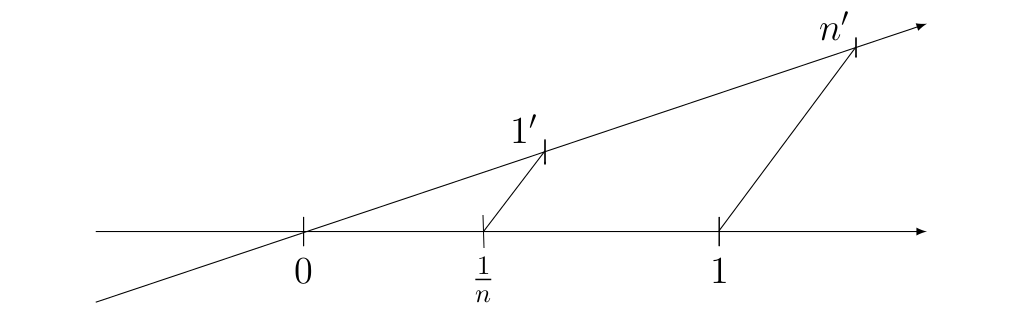
\includegraphics[width=0.8\linewidth]{falles.png}
        \end{figure}\\
        таким образом складывая $m$ раз $\frac{1}{n}$, получим любое рациональное число $\frac{m}{n}$.\\
        Построим бесконечную десятичную дробь, например $0,37152\dots$.\\
        Разобьем отрезок:
        \[\begin{tikzpicture} [scale=5.5]
        \draw[-latex] (-0.5,0) -- (1.5,0) ;
        \foreach \x in {0,0.2,0.4,0.6,0.8,1}
        \draw[shift={(\x,0)},color=black] (0pt,1pt) -- (0pt,-1pt);
        \foreach \x in {0,0.2,0.4,0.6,0.8,1}
        \draw[shift={(\x,0)},color=black] (0pt,1pt) -- (0pt,-1pt) node[below] 
        {$\x$};
        \end{tikzpicture}\]
        $0,37152\dots$ находится между $0.2$ и $0.4$, теперь разобьем этот отрезок:
        \[\begin{tikzpicture} [scale=28]
        \draw[-latex] (0.1,0) -- (0.5,0) ;
        \foreach \x in {0.2,0.24,0.28,0.32,0.36,0.4}
        \draw[shift={(\x,0)},color=black] (0pt,0.2pt) -- (0pt,0.2pt);
        \foreach \x in {0.2,0.24,0.28,0.32,0.36,0.4}
        \draw[shift={(\x,0)},color=black] (0pt,0.2pt) -- (0pt,-0.2pt) node[below] 
        {$\x$};
        \end{tikzpicture}\]
        $0,37152\dots$ находится между $0.36$ и $0.4$, теперь разобьем этот отрезок и т.д.
        Получаем последовательность вложеных отрезков, у которых длина стремится к нулю, значит у них есть единственная общая точка - наше число.\\
        Таким образом, прямая - множество бесконечных десятичных дробей, а значит на ней выполняеются (1)-(16).
        \subsection{Принципы полноты}
        \subsubsection{Верхние и нижние грани множества}
        \begin{definition} \tab
            \begin{itemize}
                \item Элемент $a\in \R$ называется максимальным элементом множества $A$\\ $(\max A\subset \R), A\ne \emptyset$, если $\forall a^{\prime}\in A: a\geq a^{\prime}$ и $a\in A$.
                \item Элемент $a\in \R$ называется минимальным элементом множества $A$\\ $(\min A\subset \R), A\ne \emptyset$, если $\forall a^{\prime}\in A: a\leq a^{\prime}$ и $a\in A$.
            \end{itemize}
        \end{definition}
        \begin{definition} \tab
            \begin{itemize}
                \item Элемент $m\in \R$ называется верхней гранью $A\subset \R, A\ne \emptyset$, если\\ $\forall a\in A: a\leq m$.
                \item Элемент $m\in \R$ называется нижней гранью $A\subset \R, A\ne \emptyset$, если\\ $\forall a\in A: a\geq m$.
            \end{itemize}
        \end{definition}
        \begin{definition} \tab
            \begin{itemize}
                \item Множество $A \subset \R, A\ne \emptyset$ называется ограниченым сверху, если у $A$ существует верхняя грань.
                \item Множество $A \subset \R, A\ne \emptyset$ называется ограниченым снизу, если у $A$ существует нижняя грань.
                \item Множество $A \subset \R$ называется ограниченым, если $A$ ограничено и сверху и снизу.
            \end{itemize}
        \end{definition}
        \begin{definition} \tab
            \begin{itemize}
                \item Пусть множество $A \subset \R$ ограничено сверху, $B$ - множество верхних граней $A$. Элемент $c=\min B$ называется точной верхней гранью $A$ и обозначается $\sup A$.
                \item Пусть множество $A \subset \R$ ограничено снизу, $B$ - множество нижних граней $A$. Элемент $c=\max B$ называется точной нижней гранью $A$ и обозначается $\inf A$.
            \end{itemize}
        \end{definition}
        \subsubsection{Принцип полноты Вейерштрасса}
        \begin{theorem} (Принцип полноты Вейерштрасса) \\
            Для каждого ограниченого сверху или снизу множества $A$ существует $\sup A$ или $\inf A$ соответственно.
        \end{theorem}
        \begin{proof}
            Докажем для верхней грани (аналогично для нижней)\\
            $A$ - ограничено сверху, $B$ - множество верхних граней. Значит $\forall a\in A$ и \\$\forall b\in B: a\leq b \Rightarrow$ по аксиоме полноты $\exists\ c\in \R: a\leq c\leq b \Rightarrow c=\sup A$.
        \end{proof}\newpage
        \begin{definition}
            $\forall a,b\in \R: a<b$ рассмотрим следующие множетсва:
            \begin{itemize}
                \item $[a,b] := \{x\in \R: a\leq x\leq b\}$ - отрезок
                \item $(a,b) := \{x\in \R: a<x<b\}$ - интервал
                \item $[a,b) := \{x\in \R: a\leq x<b\}$ - полуинтервал
                \item $(a,b] := \{x\in \R: a<x\leq b\}$ - полуинтервал
            \end{itemize}
            Такие множества называют промежутками.
        \end{definition} 
        \begin{definition}
            $\forall a\in \R$ функция
            \[|a|=
                \begin{cases}
                    \tab[12pt]a, \tab[5pt] a\geq 0,\\
                    -a, \tab[5pt] a<0.
                \end{cases}\]
            называется модулем.
        \end{definition}
        \begin{definition}
            Для любого промежутка с концами $a,b\in \R$ длиной называется число $|b-a|$.
        \end{definition}
        \begin{definition}
            Рассмотрим последовательность $\{[a_n,b_n]\}_{n=1}^{\infty}$. Говорят, что\\ $|b_n-a_n|\to 0$ при $n\to \infty$, если $\forall \epsilon >0\tab[5pt]\exists N\in \N: \forall n>N$ выполнено $|b_n-a_n|<\epsilon$.
        \end{definition}
        \subsubsection{Принцип вложеных отрезков (принцип полноты Кантора)}
        \begin{theorem} (Принцип вложеных отрезков) \\
            Пусть последовательность $\{[a_n,b_n]\}_{n=1}^{\infty}$ такова, что $\forall n: [a_{n+1},b_{n+1}]\subset [a_n,b_n]$. Тогда $\exists c\in \R: c\in [a_n,b_n], \forall n$. Если $|b_n-a_n|\to 0$ то $c$ - единственная.
        \end{theorem} 
        \begin{proof}
            $\forall n,m\in \N: a_n\leq b_m$, т.к
            \begin{itemize}
                \item если $n<m$, то $a_n\leq a_m\leq b_m$.
                \item если $n>m$, то $a_n\leq b_n\leq b_m$.
            \end{itemize}
            Значит для $\forall m,n\in \N: $
            Рассмотрим множества $A=\{a_n\}$ и $B=\{b_n\}$. По аксиоме полноты $\exists c\in \R: a_n\leq c\leq b_m,\ \forall n,m \Rightarrow a_n\leq c\leq b_n,\ \forall n$.\\
            Пусть $|b_n-a_n|\to 0$, предположим, что $\exists\ c_1$ и $c_2: c_1\ne c_2$ - различные общие точки, значит $|c_2-c_1|>0$. Получаем, что $0<|c_2-c_1|<|b_n-a_n|,\ \forall n$, значит $|c_2-c_1|\to 0$ получаем противоречие.
        \end{proof}
        \subsection{Неравенство Бернулли и Бином Ньютона}
        \begin{theorem} (Неравенство Бернулли)\\
            Пусть $\{x_k\}_{k=1}^n, x_k\in \R \tab[3pt] \forall k: x_k>0$ или $x_k\in (-1, 0)$. Тогда
            \[\prod\limits_{k=1}^n(1+x_k)\geq 1+\sum\limits_{k=1}x_k\]
        \end{theorem} 
        \begin{proof}
            Индукция по $n$.
            База: $n=1: 1+x_1\geq 1+x_1$.
            Пусть при $n$ утверждение верно.
            \[\prod\limits_{k=1}^{n+1}(1+x_n)\geq(1+x_{n+1})(1+\sum\limits_{k=1}^nx_k)=1+\sum\limits_{k=1}^{n+1}x_k+(\sum\limits_{k=1}^{n}x_k)\cdot x_{n+1}> 1+\sum\limits_{k=1}^{n+1}x_n\]
        \end{proof}
        \begin{definition}
            Число $\frac{n!}{k!(n-k)!}$ называется биномиальным коэффициентом и обозначается $C_n^k$.
        \end{definition} 
        \begin{comm}
            По определнию считается, что $0!=1$.
        \end{comm} 
        \begin{theorem} (Бином Ньютона)
            \[(a+b)^n=\sum\limits_{k=0}^n C_n^k a^k b^{n-k}\]
        \end{theorem} 
        \begin{proof}
            Индукция по $n$. База: для $n=1$ верно. Пусть верно для $n$. Распишем выражение для $n+1$:
            \[(a+b)^{n+1}=(a+b)\sum\limits_{k=0}^n C_n^k a^k b^{n-k}=\sum\limits_{k=0}^n C_n^k a^{k+1} b^{n-k}+\sum\limits_{k=0}^n C_n^k a^k b^{n-k+1}\]
            Сдвинем нумерацию в первой сумме:
            \[\sum\limits_{k=0}^n C_n^k a^{k+1} b^{n-k}=\sum\limits_{m=1}^n C_n^{m-1} a^{m} b^{n-m+1}\]
            Получаем, что
            \begin{multline*}
            \sum\limits_{k=0}^n C_n^k a^{k+1} b^{n-k}+\sum\limits_{k=0}^n C_n^k a^k b^{n-k+1}=\sum\limits_{m=1}^n C_n^{m-1} a^{m} b^{n-m+1}+\sum\limits_{m=0}^n C_n^m a^m b^{n-m+1}=\\=C_n^n a^{n+1}b^0+\sum\limits_{m=1}^n(C_n^{m-1}+C_n^m)a^n b^{n-m+1}+C_n^0a^0b^{n+1}=\sum\limits_{m=0}^{n+1}C_{n+1}^m a^m b^{n-m+1}
            \end{multline*}
        \end{proof} 
        \subsection{Отношение эквивалентности. Равномощные множества}
        \begin{definition}
            Отношение $\sim$ называется отношением эквивалентности, если оно удовлетворяет:
            \begin{enumerate}
                \item $x\sim x$ (Рефлексивность)
                \item $x\sim y \Rightarrow y\sim x$ (Симметричность)
                \item $x\sim y$ и $y\sim z\Rightarrow x\sim z$ (Транзитивность)
            \end{enumerate}
        \end{definition} 
        \begin{definition}
            Множества называются равномощными, если между ними существует биекция.
        \end{definition}
        \begin{theorem}
            Равномощность множеств является отношением эквивалентности.
        \end{theorem}
        \begin{proof} Пусть $A,B,C$ - множества, $\phi:A\to B, \psi:B\to C$ - биекции.
            \begin{enumerate}
                \item Рефлексивность очевидна, поскольку у любого множества существует биекция в себя.
                \item Для любой биекции $\phi:A\to B$ существует $\phi^{-1}:B\to A$.
                \item $\phi:A\to B, \psi:B\to C$, то $\phi \circ \psi: A\to C$.
            \end{enumerate}
        \end{proof} 
        \begin{theorem}
            Конечные множества равномощны $\lra$ они содержат одинаковое количество элементов.
        \end{theorem}
        \begin{proof}
            \begin{itemize}
                \item[$(\Leftarrow)$] Пусть $\phi:A\to \{1,\dots, n\}, \ \psi:B\to \{1,\dots, n\}\\
                \Rightarrow \exists \ \psi^{-1}:\{1,\dots, n\}\to B$. Тогда $\phi \circ \psi^{-1}:A\to B$ - искомая биекция.
                \item[$(\Rightarrow)$] Пусть $\phi:A\to B$ - биекция. Если $A=\emptyset$, то $B=\emptyset$. Докажем индукцией по количеству элементов. Пусть $A=\{a\}$, тогда $\exists \ b\in B: \phi(a)=b$. Пусть утверждение верно для случая когда $A$ - $n$-элементное множество. Теперь если $A$ - $n+1$-элементное, то $\exists \ \phi:A\to \{1,2,...,n+1\}$ - биекция. Значит $\exists \ a\in A$, что $\phi(a)=n+1$. Тогда $A\setminus\{a\}$ - $n$-элементное. Также $\exists \ b\in B: b=\phi(a) \Rightarrow B\setminus\{b\}$ - $n$-элементное $\Rightarrow  B$ - $n+1$-элементное.
            \end{itemize}
        \end{proof}
        \begin{definition}
            Множества равномощные $\N$ называются счетными.
        \end{definition}
        \begin{theorem}
            $A_i$ - счетные множества $\Rightarrow \bigcup\limits_{n=1}^{\infty}A_i$ - счетно.
        \end{theorem}
        \begin{proof}
            Предъявим проход по элементам, который задает биекцию:
            \begin{center}
                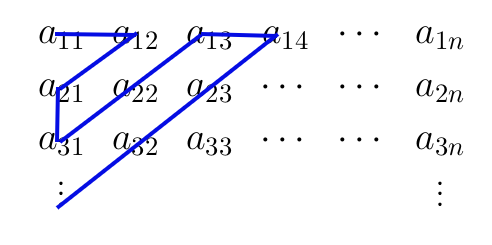
\includegraphics[width=0.4\linewidth]{prohod.png}
            \end{center}
        \end{proof}
        \begin{definition}
            Множество называется не более чем счетным, если оно конечно или счетно.
        \end{definition}
        НЕ БОЛЕЕ ЧЕМ СЧЕТНОЕ ОБЪЕДИНЕНИЕ НЕ БОЛЕЕ ЧЕМ СЧЕТНЫХ МНОЖЕСТВ НЕ БОЛЕЕ ЧЕМ СЧЕТНО (ДОПИСАТЬ) 
        \begin{examples}
            \begin{enumerate}\tab
                \item Множество целых чисел $\Z$
                \item Множество рациональных чисел $\Q$
                \item Множество многочленов с рациональными коэффициентами.
                \item Множество алгебраических чисел (чисел которые являются корнями многочлена с рациональными коэффициентами).
            \end{enumerate}
        \end{examples}
        \subsection{Теорема Кантора и аксиома выбора}
        \begin{theorem} (Теорема Кантора)\\
            Множество бесконечных последовательностей, состоящих из нулей и единиц несчетно.
        \end{theorem} 
        \begin{proof}
            Предположим, что оно счетно. Тогда все последовательности нулей и единиц можно перенумеровать. Составим бесконечную вниз таблицу, строками которой будут наши последовательности:\\
            \tab[6cm]$a_1=\underline{a_{11}}\ a_{12}\ a_{13}\ a_{14}\ \dots$\\
            \tab[6cm]$a_2=a_{21}\ \underline{a_{22}}\ a_{23}\ a_{24}\ \dots$\\
            \tab[6cm]$a_3=a_{31}\ a_{32}\ \underline{a_{33}}\ a_{34}\ \dots$\\
            \tab[6cm]$a_4=a_{41}\ a_{42}\ a_{43}\ \underline{a_{44}}\ \dots$\\
            \tab[6cm]\vdots\\
            $a_{ij}$ - $j$-й член $i$-й последовательности. Рассмотрим последовательность $b$ у которой $b_i=1-a_{ii}$. Такая последовательность отличается от каждой $i$-й последовательности на $i$-й позицции, значит она не была посчитана, получаем противоречие.
        \end{proof}
        \begin{statement}
            \begin{enumerate}\tab
                \item Алгебраических чисел счетно.
                \item Действительных чисел несчетно.
            \end{enumerate}
        \end{statement}
        \begin{definition}
            Действительные числа не являющееся алгебраическими называются трансцендентными.
        \end{definition} 
        \begin{definition}
            Множества равномощные множеству последовательностей нулей и единиц называются множествами мощности континуума.
        \end{definition} 
        \begin{theorem}
            У любого множетсва мощность множества всех подмножеств строго больше чем мощность самого множества.
        \end{theorem}
        \begin{definition}
            Для множеств $A$ и $B$ обозначим $|A|\leq |B|$, если $\exists \ B^{\prime} \subset B$ для которого $\exists \ \phi:A\to B^{\prime}$ - биекция.
        \end{definition} 
        \begin{theorem}
            Сравнение мощностей множеств $|A|\leq |B|$ является отношением порядка.
            \begin{enumerate}
                \item $\forall A,B: |A|\leq |B|$ или $|B|\leq |A|$ 
                \item $|A|\leq |B|$ и $|B|\leq |A| \Rightarrow |A|=|B|$
                \item $|A|\leq |B|$ и $|B|\leq |C| \Rightarrow |A|\leq |C|$
            \end{enumerate}
        \end{theorem}
        \begin{proof}
            Без доказательства.
        \end{proof}
        \begin{axiom}(Аксиома выбора)\\
            Если существует множетсво неких множеств, то из каждоко множества можно выбрать по одному элементу и составить из них другое множество.
        \end{axiom}
        \begin{statement}
            Множество всех подмножеств $\N$ равномощно множеству бесконечных последовательностей нулей и единиц.
        \end{statement}
        \begin{proof}
            Каждому $A\subset \N$ ставим в соответствие характеристическую последовательность, которая принимает значения: единицу, если элемент лежит в подмножестве и ноль иначе.
        \end{proof}
        \begin{theorem}
            У любого бесконечного множества существует счетное подмножество.
        \end{theorem} 
        \begin{proof}
            Выбираем элемент и сразу присваиваем ему номер, продолжая это действие, построим счетное множество.
        \end{proof}
        \begin{theorem}
            Пусть $A$ - бесконечное, $B$ - не более чем счетное $\Rightarrow A\sim A\cup B$
        \end{theorem} 
        \begin{proof}
            Пусть $A^{\prime}\subset A$. Тогда $A\sim (A\setminus A^{\prime})\cup A^{\prime}\sim (A\setminus A^{\prime})\cup(A^{\prime}\cup B)\sim\\ \sim(A\cup B)$.
        \end{proof}
    \section{Топология $\R$}
        \begin{definition}
            $\forall x\in \R \ \forall \epsilon>0$ отрезок $B_{\epsilon}(x)=(x-\epsilon, x+\epsilon)$ называется\\ $\epsilon$-окрестностью точки $x$.
        \end{definition}
        \begin{definition}
            $\forall x\in \R \ \forall \epsilon>0$ отрезок $\mathring{B}_{\epsilon}(x)=(x-\epsilon,x)\cup(x,x+\epsilon)$ называется проколотой $\epsilon$-окрестностью точки $x$.
        \end{definition} 
        \begin{definition}
            Точка $x\in A\subset \R$ называется внутренней точкой множества $A$, если $\exists \ B_{\epsilon}(x)\subset A$. Множество всех внутренних точек $x\in A$ называется внутренностью множетсва $A$.
        \end{definition} 
        \begin{definition}
            Точка $x\in \R\setminus A$ называется внешней точкой для множества $A\subset \R$, если $x$ - внутренняя точка для $\R\setminus A$. Множество всех внешних точек $x\in A$ называется внешностью множетсва $A$.
        \end{definition}
        \begin{definition}
            Точка называется граничной для множества $A\subset \R$, если она не является ни внешней ни внутренней для $A$. Множество всех граничных точек называется границей и обозначается $\partial A$.
        \end{definition}
        \begin{definition} (Множество Кантора)\\
            Разбиваем отрезок $[0,1]$ на три части и выбрасываем середину, затем каждый из получившихся отрезков разбиваем на три части и выбрасываем середину, и т.д.
            \begin{itemize}
                \item Суммарная длина всех выброшеных интервалов равна $1$.
                \item Концов отрезков счетное множество.
                \item Общее количество точек имеет мощность континуума.
            \end{itemize}
        \end{definition} 
        \begin{definition}
            Множество называется открытым, если все его точки внутренние.
        \end{definition}
        \begin{comm}
            Любой интервал - открытое множество
        \end{comm}
        \begin{definition}
            Множество называется $A\subset \R$ замкнутым, если все его дополнение $\R\setminus A$ открыто.
        \end{definition} 
        \begin{comm}
            Отрезок - и не открытое и не замкнутое множество.
        \end{comm}
        \begin{comm}
            По определению считаем, что $\emptyset$ и $\R$ и открыты и замкнуты одновременно.
        \end{comm} 
        \begin{definition}
            Точка $x\in \R$ называется передельной точкой множества $A\subset \R$, если в любой проколотой окрестности точки $x$ бесконечно много точек $A$, т.е\\
            $\forall \epsilon >0\ A\cap \mathring{B}_{\epsilon}(x)\ne\emptyset$.
        \end{definition} 
        \begin{definition}
            Точка $x\in A$ называется изолированной точкой $A\subset \R$, если $\exists \ \epsilon>0: A\cap \mathring{B}_{\epsilon}(x)=\emptyset$.
        \end{definition} 
        \begin{definition}
            Точка $x\in \R$ называется точкой прикосновения $A\subset \R$, если $\forall \ \epsilon>0: A\cap {B}_{\epsilon}(x)\ne\emptyset$.
        \end{definition} 
\end{document}